\section{真实排版案例}
下面四个案例使用各自的文档类实际编译，效果与完整源码均收录于本手册。
配套源码位于 \key{docs/layouts}；使用构建脚本编译会自动搜索 \key{sty/gradbars.sty}。
这些是实际排版环境，所有数值仍为演示数据。

\subsection{示例 74：双栏论文}
使用 article 的 twocolumn 选项；数据条宽度按单栏分配。
下图是完整双栏页面。窄列的总宽度还需加上外部标签槽与间隔。
\begin{center}
\fbox{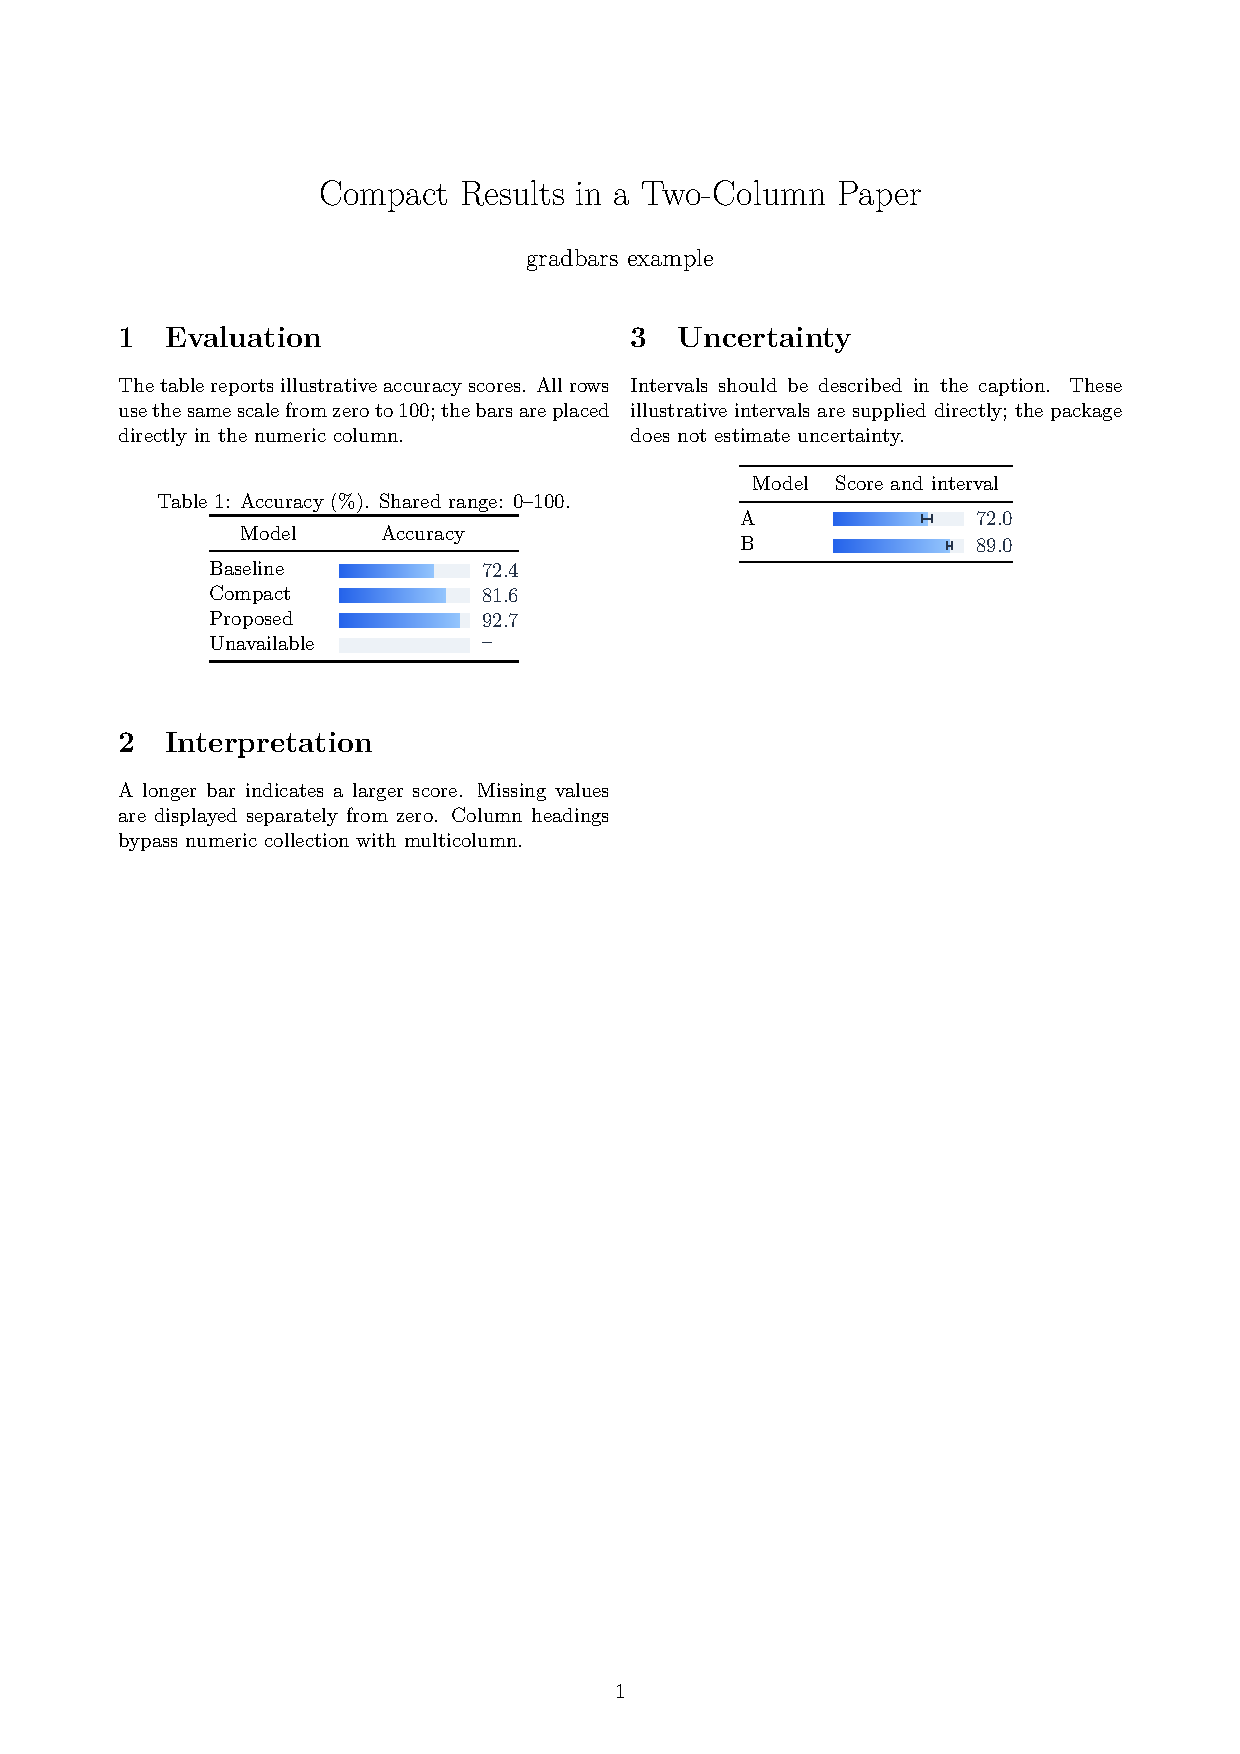
\includegraphics[width=.84\linewidth,height=.72\textheight,keepaspectratio]{docs/layouts/twocolumn.pdf}}
\end{center}
\clearpage
\textbf{示例 74 完整源码}\par
\lstinputlisting[style=manual]{docs/layouts/twocolumn.tex}

\clearpage
\subsection{示例 75：跨页长表}
longtable 在单栏文档中自动分页，并在后续页重复表头。
该案例包含 60 行，实际输出两页。所有页面使用相同的列定义和 0--100 量程。
\begin{center}
\fbox{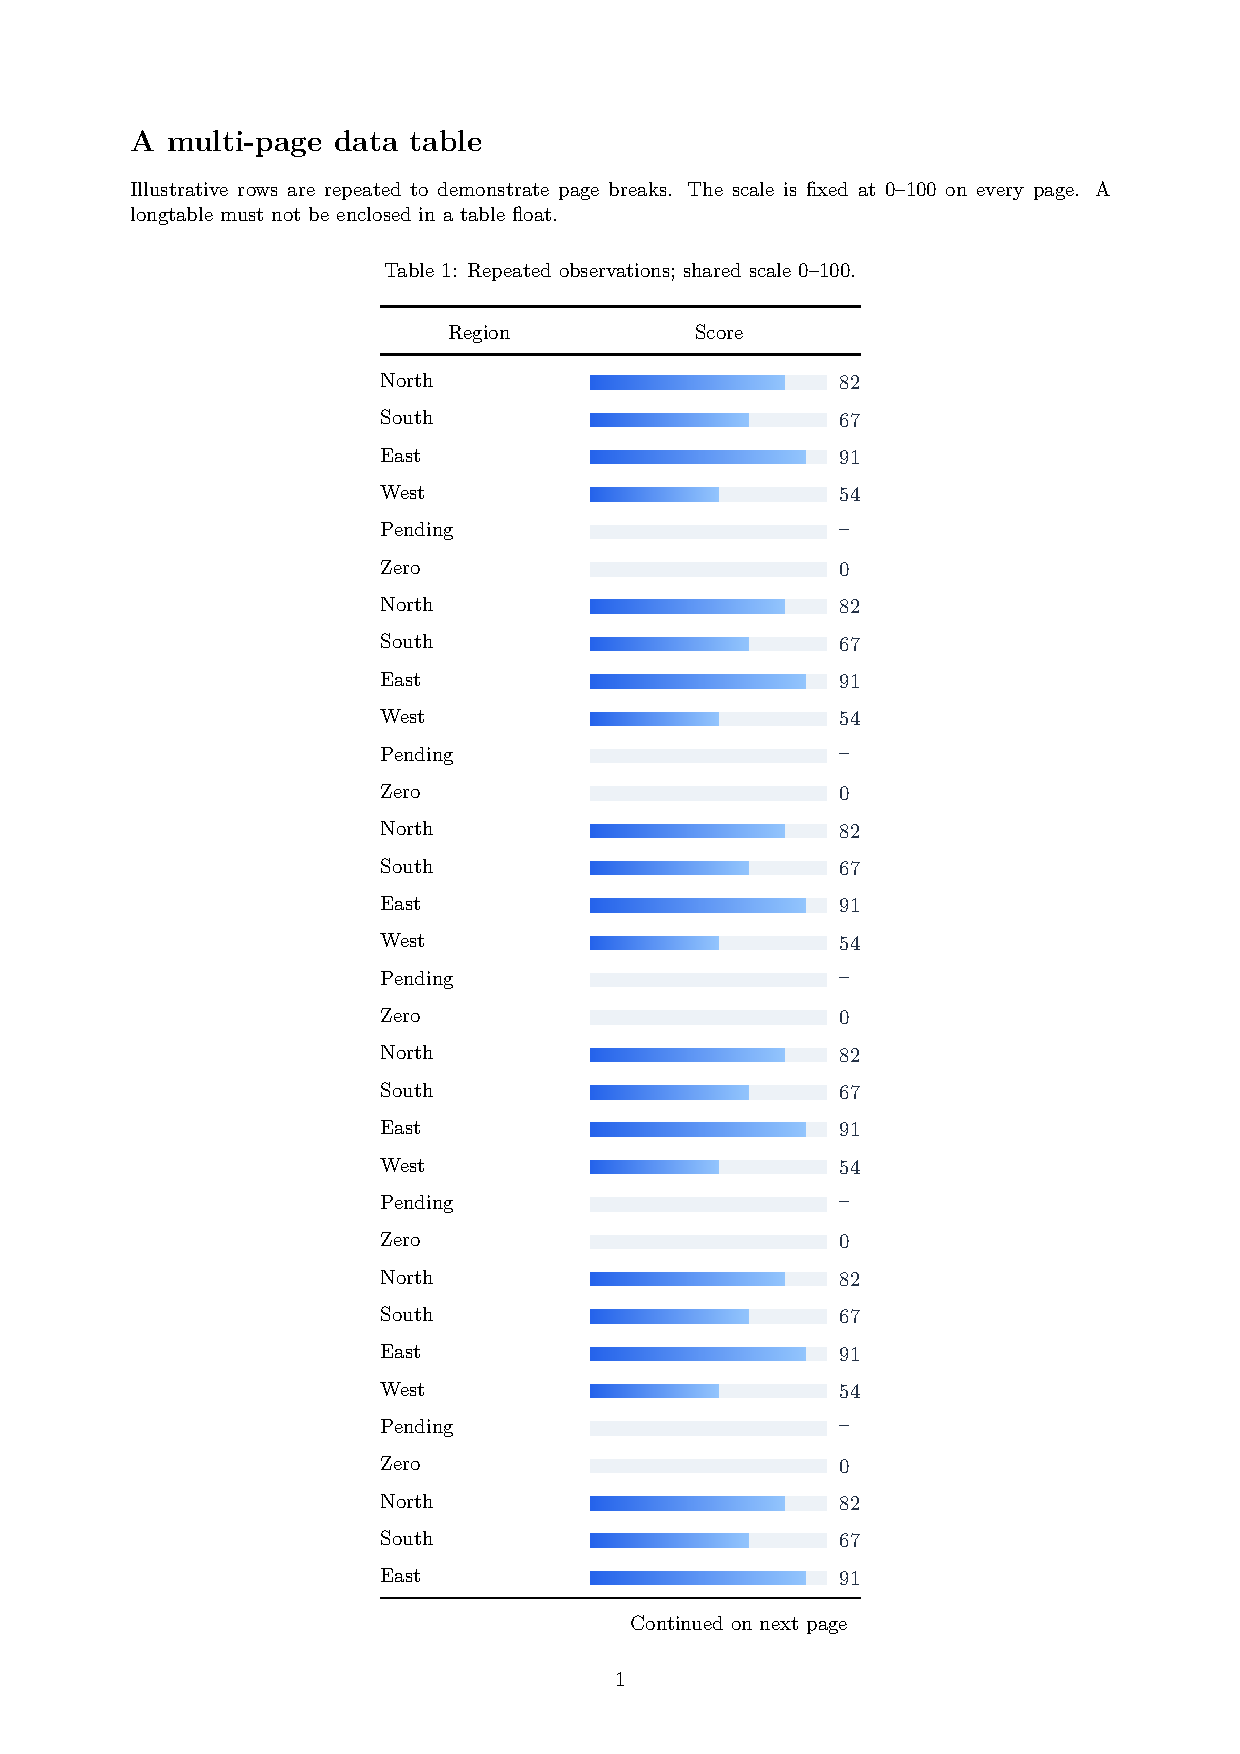
\includegraphics[page=1,width=.46\linewidth]{docs/layouts/longtable.pdf}}
\hfill
\fbox{\includegraphics[page=2,width=.46\linewidth]{docs/layouts/longtable.pdf}}
\end{center}
长表不能放在 table 浮动体内，也不能直接用在 article 的双栏模式中。
需要跨页时，将这部分切换为单栏或单独编排。
\clearpage
\textbf{示例 75 完整源码}\par
\lstinputlisting[style=manual,basicstyle=\ttfamily\fontsize{7.5}{9}\selectfont]{docs/layouts/longtable.tex}

\clearpage
\subsection{示例 76：黑白打印}
使用灰度主题与不同灰度的分段，同时保留数值、图例名称和目标线。
下图截取实际页面的内容区域，堆叠条与图例同时使用黑白纹理。
\begin{center}
\fbox{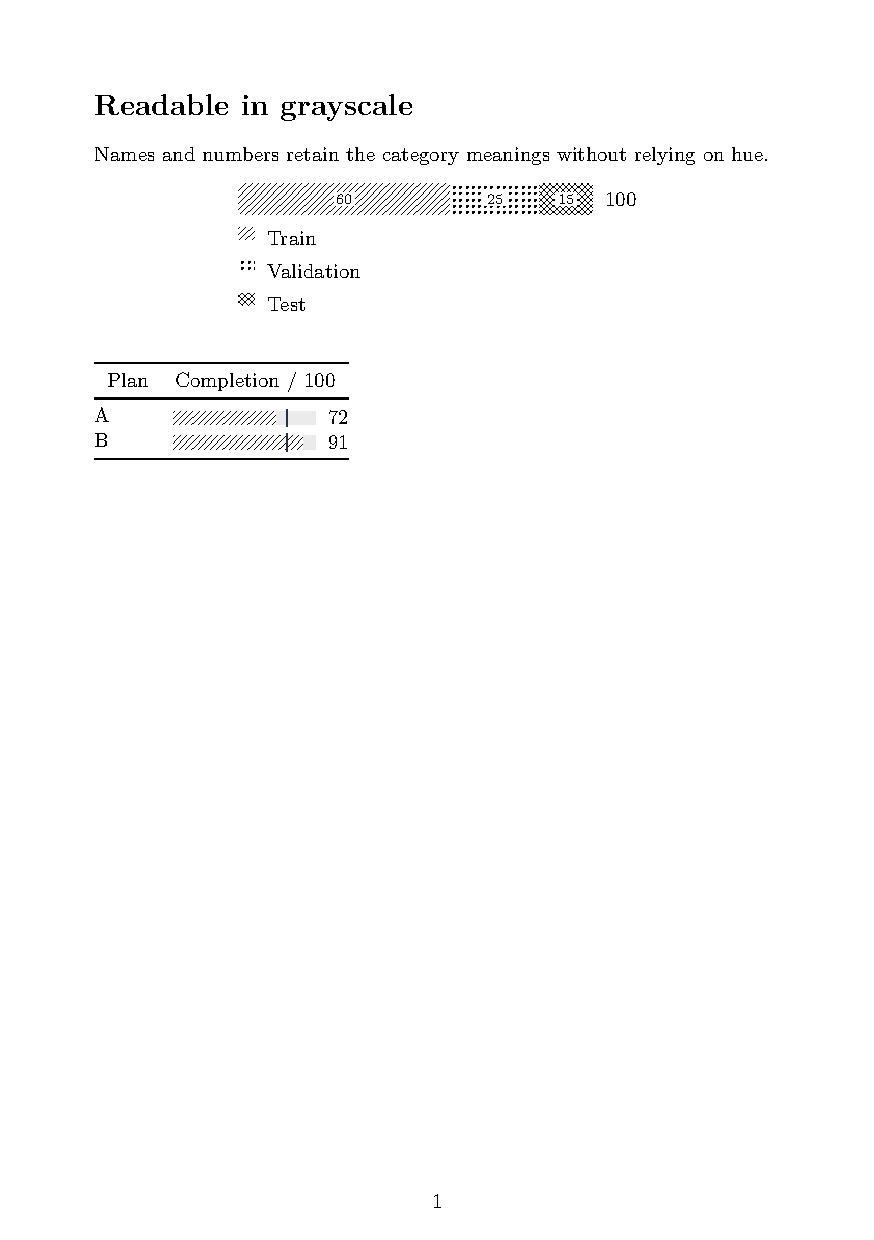
\includegraphics[trim=35bp 360bp 35bp 35bp,clip,width=.72\linewidth]{docs/layouts/grayscale.pdf}}
\end{center}
\textbf{示例 76 完整源码}\par
\lstinputlisting[style=manual]{docs/layouts/grayscale.tex}

\clearpage
\subsection{示例 77：幻灯片}
使用 Beamer 的 16:9 页面。增大轨道高度，并通过 arraystretch 增加表格行距，
使标签和相邻条形之间保留空隙。若幻灯片内还要显示 verbatim 源码，需给 frame 添加 fragile。
\begin{center}
\fbox{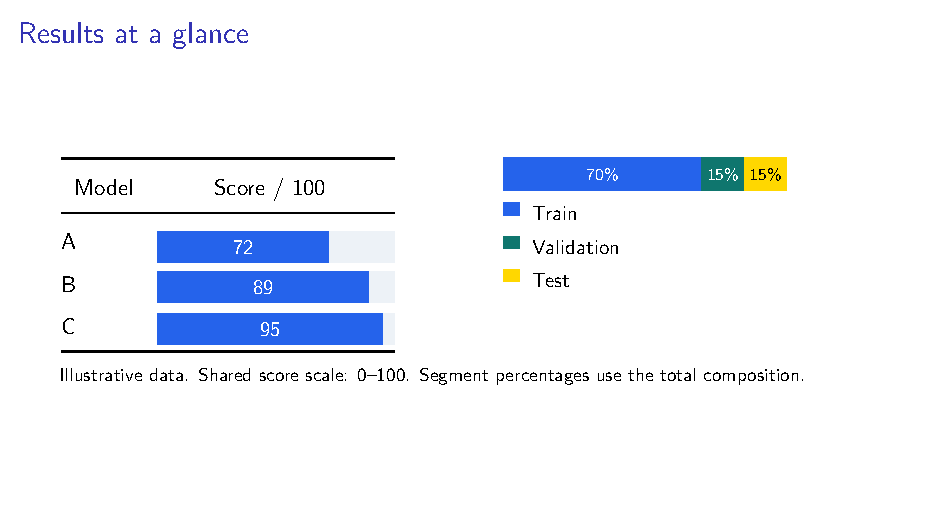
\includegraphics[width=.92\linewidth]{docs/layouts/slides.pdf}}
\end{center}
\textbf{示例 77 完整源码}\par
\lstinputlisting[style=manual,basicstyle=\ttfamily\fontsize{7.5}{8.5}\selectfont]{docs/layouts/slides.tex}
